% SC3020 --- Chapter 2: Data Preprocessing (0->100 ground-up)
\chapter{Data Preprocessing}
\label{ch:preprocessing}

\begin{quote}
\emph{``Garbage in, garbage out.''} No algorithm rescues bad inputs. Preprocessing --- cleaning, transforming, and reducing data --- is where most projects succeed or fail.
\end{quote}

\noindent\fbox{\parbox{\dimexpr\linewidth-2\fboxsep-2\fboxrule}{%
\textbf{From zero: no preprocessing assumed.} We start from a messy spreadsheet with missing cells and strange outliers, explain why each defect hurts models, then formalise cleaning, normalisation, and reduction. Pictures precede equations.}}
\vspace{0.4em}

\section*{Learning Outcomes}
After this chapter you will be able to:
\begin{enumerate}[label=(L\arabic*)]
    \item diagnose missingness mechanisms (MCAR/MAR/MNAR) and choose imputation strategies;
    \item apply normalisation (min-max, $z$-score, robust) and explain when each fails;
    \item handle outliers and noisy data with binning, clipping, and regression smoothing;
    \item reduce dimensionality via feature selection, sampling, and PCA intuition;
    \item build a reproducible preprocessing pipeline in Python.
\end{enumerate}

% ============================================================
\section{Why Preprocessing Dominates}
\label{sec:why-preprocess}
\paragraph{Intuition.} Imagine training a loan model where 20\% of incomes are blank, one entry reads ``age = 231,'' and salary is in dollars while age is in years. Distance-based learners (kNN, k-means) will be dominated by salary; a single outlier can flip a mean; missing values crash most code. Real data is incomplete, noisy, and inconsistent because it comes from humans, sensors, and merged systems.

\paragraph{Quality dimensions.} Accuracy (correct values), completeness (no missing), consistency (no contradictions), timeliness (up-to-date), and interpretability. A \emph{preprocessing pipeline} chains operations $T_k\circ\cdots\circ T_1(\mathcal{D})$ that map raw $\mathcal{D}$ to analysis-ready $\mathcal{D}'$ while preserving signal and documenting every choice for reproducibility.

% ============================================================
\section{Cleaning: Missing Values and Noise}
\label{sec:cleaning}
\paragraph{Missingness.} Mechanisms: \emph{MCAR} (missing completely at random, e.g., sensor glitch independent of data), \emph{MAR} (missing depends on observed data, e.g., higher incomes less likely to be reported), \emph{MNAR} (missing depends on the missing value itself, e.g., people with very high debt hide it). Strategies: row/column deletion (only if MCAR and few), mean/median/mode imputation, regression or $k$NN imputation, and model-based (EM). Deletion under MAR/MNAR biases results.

\paragraph{Noise and outliers.} \emph{Binning} (equal-width, equal-frequency, then smooth by mean/median/boundary), \emph{regression smoothing}, \emph{clipping} (winsorisation), and \emph{clustering}: points far from any cluster are candidate outliers. Rule-of-thumb: $|z|>3$ flags a univariate outlier; multivariate needs Mahalanobis distance or isolation forest.

\begin{figure}[h]\centering
\begin{tikzpicture}[scale=0.92, every node/.style={font=\scriptsize}]
% Before: messy scatter with outlier and missing marks
\node[font=\footnotesize\bfseries] at (2.2,3.2) {Before preprocessing};
\draw[thick, gray!50] (0,0) rectangle (4.4,2.6);
\draw[->, thick] (0,0)--(4.8,0) node[right, font=\tiny] {age};
\draw[->, thick] (0,0)--(0,3.0) node[above, font=\tiny] {income};
\foreach \x/\y in {0.6/0.5, 1.0/0.8, 1.4/1.0, 1.8/1.2, 2.2/1.5, 2.6/1.7, 3.0/1.9, 3.4/2.0} \fill[blue!60!black] (\x,\y) circle (1.6pt);
\fill[red!70!black] (4.0,2.5) circle (2.2pt) node[above right, font=\tiny, fill=red!10, rounded corners=1pt, inner sep=1pt] {outlier};
\node[font=\tiny, fill=yellow!14, rounded corners=2pt, inner sep=2pt] at (2.2,-0.55) {scale dominates; outlier skews mean};
% missing marks
\node[font=\tiny, fill=orange!14, draw, rounded corners=2pt, inner sep=2pt] at (1.0,2.9) {? = missing};
% After
\node[font=\footnotesize\bfseries] at (8.4,3.2) {After cleaning + normalisation};
\draw[thick, gray!50] (6.2,0) rectangle (10.6,2.6);
\draw[->, thick] (6.2,0)--(11.0,0) node[right, font=\tiny] {age ($z$-score)};
\draw[->, thick] (6.2,0)--(6.2,3.0) node[above, font=\tiny] {income ($z$-score)};
\foreach \x/\y in {6.9/0.9, 7.2/1.0, 7.5/1.15, 7.9/1.25, 8.3/1.45, 8.7/1.55, 9.0/1.75, 9.4/1.85} \fill[green!55!black] (\x,\y) circle (1.6pt);
\fill[green!55!black] (10.1,2.1) circle (1.6pt) node[above right, font=\tiny, fill=green!10, rounded corners=1pt, inner sep=1pt] {clipped};
\node[font=\tiny, fill=green!12, rounded corners=2pt, inner sep=2pt] at (8.4,-0.55) {comparable scales; outlier handled; imputed};
\draw[-{Latex[length=3mm]}, thick, blue!60!black] (4.7,1.3)--(5.9,1.3) node[midway, above, font=\tiny, fill=blue!8, rounded corners=2pt, inner sep=2pt] {pipeline};
\end{tikzpicture}
\caption{Preprocessing effect. Left: raw data with an outlier and missing marker; right: after imputation, clipping, and standardisation, both features contribute comparably.}
\label{fig:cleaning-before-after}
\end{figure}

% ============================================================
\section{Transformation: Normalisation and Discretisation}
\label{sec:transformation}
\paragraph{Intuition.} If one feature ranges $[0,10000]$ and another $[0,1]$, Euclidean distance is just the first feature. Normalisation puts features on comparable footing; discretisation turns numbers into bins when algorithms need categories.

\paragraph{Formal methods.} For feature $x$ with min $x_{\min}$, max $x_{\max}$, mean $\mu$, std $\sigma$:
\begin{align}
\text{Min-max:}&\quad x' = \frac{x-x_{\min}}{x_{\max}-x_{\min}}\in[0,1],
& \text{sensitive to outliers.} \label{eq:minmax}\\
\text{Z-score:}&\quad x' = \frac{x-\mu}{\sigma}\quad (\mu_{x'}=0,\ \sigma_{x'}=1),
& \text{assumes roughly Gaussian.} \label{eq:zscore}\\
\text{Robust:}&\quad x' = \frac{x-\text{median}}{\text{IQR}},\quad \text{IQR}=Q_3-Q_1,
& \text{outlier-resistant.} \label{eq:robust}
\end{align}
Decimal scaling ($x/10^j$) and log transforms handle heavy tails. \emph{Discretisation}: equal-width (cut range into $k$ intervals), equal-frequency (each bin has $n/k$ points), and entropy-based (choose cuts that maximise class separation). Normalise \emph{after} splitting into train/test to avoid leakage.

\begin{figure}[h]\centering
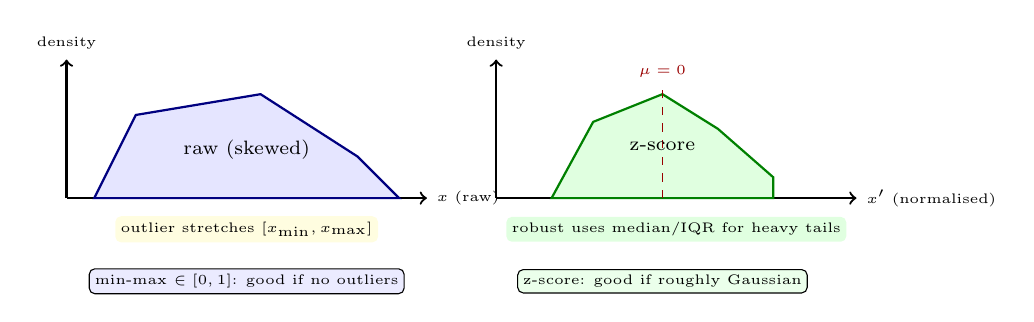
\begin{tikzpicture}[scale=0.88, every node/.style={font=\scriptsize}]
% Min-max vs z-score illustration
\draw[->, thick] (0,0)--(5.2,0) node[right, font=\tiny] {$x$ (raw)};
\draw[->, thick] (0,0)--(0,2.0) node[above, font=\tiny] {density};
\draw[thick, fill=blue!10, draw=blue!50!black] (0.4,0)--(1.0,1.2)--(2.8,1.5)--(4.2,0.6)--(4.8,0) -- cycle;
\node at (2.6,0.7) {raw (skewed)};
\node[font=\tiny, fill=yellow!12, rounded corners=2pt, inner sep=2pt] at (2.6,-0.45) {outlier stretches $[x_{\min},x_{\max}]$};

\draw[->, thick] (6.2,0)--(11.4,0) node[right, font=\tiny] {$x'$ (normalised)};
\draw[->, thick] (6.2,0)--(6.2,2.0) node[above, font=\tiny] {density};
% z-score roughly centred
\draw[thick, fill=green!12, draw=green!50!black] (7.0,0) -- (7.6,1.1) -- (8.6,1.5) -- (9.4,1.0) -- (10.2,0.3) -- (10.2,0) -- cycle;
\draw[dashed, red!60!black] (8.6,0)--(8.6,1.6) node[above, font=\tiny] {$\mu=0$};
\node at (8.6,0.75) {z-score};
\node[font=\tiny, fill=green!12, rounded corners=2pt, inner sep=2pt] at (8.8,-0.45) {robust uses median/IQR for heavy tails};
% legend
\node[font=\tiny, fill=blue!8, draw, rounded corners=2pt, inner sep=2pt] at (2.6,-1.2) {min-max $\in[0,1]$: good if no outliers};
\node[font=\tiny, fill=green!8, draw, rounded corners=2pt, inner sep=2pt] at (8.6,-1.2) {z-score: good if roughly Gaussian};
\end{tikzpicture}
\caption{Normalisation choices. Min-max preserves distribution shape but an outlier compresses all other points; $z$-score centres at zero; robust scaling survives outliers.}
\label{fig:normalisation}
\end{figure}

\begin{lstlisting}[language=Python, caption={A reproducible pipeline: impute, handle outliers, scale --- fit on train only.}, label={lst:preprocess}]
import pandas as pd, numpy as np
from sklearn.model_selection import train_test_split
from sklearn.impute import SimpleImputer
from sklearn.preprocessing import StandardScaler, RobustScaler

df = pd.DataFrame({"age":[25,30,np.nan,231,45], "income":[40,55,60,65,200]})
# Correct split BEFORE fitting transformers (avoid leakage)
train, test = train_test_split(df, test_size=0.3, random_state=0)

# 1. Impute (median resists the 231 outlier)
imp = SimpleImputer(strategy="median")
train_imp = imp.fit_transform(train)      # fit on train only
test_imp  = imp.transform(test)           # apply to test

# 2. Clip univariate outlier (|z|>3) -- simple winsorisation
def winsorise(X, k=3):
    mu, sd = X.mean(axis=0), X.std(axis=0, ddof=0)
    return np.clip(X, mu - k*sd, mu + k*sd)
train_clip = winsorise(train_imp)

# 3. Scale
scaler = StandardScaler()                 # or RobustScaler for heavy tails
train_scaled = scaler.fit_transform(train_clip)
test_scaled  = scaler.transform(test_imp)
print(train_scaled.mean(axis=0), train_scaled.std(axis=0))
\end{lstlisting}

% ============================================================
\section{Reduction: Selecting and Compressing}
\label{sec:reduction}
\paragraph{Intuition.} Hundreds of features slow learners, add noise, and invite overfitting (curse of dimensionality). Reduction keeps signal, drops redundancy.

\paragraph{Families.} \emph{Feature selection}: filter (rank by correlation/mutual information), wrapper (search subsets, evaluate with model), embedded (LASSO, tree importance). \emph{Feature extraction}: create new features, e.g., \emph{PCA} (find orthogonal directions of maximal variance; project onto top $k$). Intuition: if data lie near a line in $\mathbb{R}^2$, PCA rotates axes so one coordinate captures almost all variance. \emph{Sampling}: row reduction (random, stratified), and \emph{data cube aggregation} (roll-up). \emph{Numerosity}: replace data by parameters (regression) or histograms.

\begin{figure}[h]\centering
\begin{tikzpicture}[scale=0.9, every node/.style={font=\scriptsize}]
% PCA intuition: cloud with principal axis
\draw[->, thick] (0,0)--(4.6,0) node[right, font=\tiny] {$x_1$};
\draw[->, thick] (0,0)--(0,3.2) node[above, font=\tiny] {$x_2$};
\foreach \x/\y in {1.0/0.8,1.2/1.0,1.5/1.2,1.7/1.4,2.0/1.6,2.2/1.7,2.5/2.0,2.7/2.1,3.0/2.4,3.2/2.5} \fill[blue!60!black] (\x,\y) circle (1.4pt);
\draw[thick, red!65!black, -{Latex[length=2.5mm]}] (0.6,0.5)--(3.8,2.8) node[midway, above, sloped, font=\tiny, fill=red!10, rounded corners=1pt, inner sep=2pt] {PC1 (max variance)};
\draw[thick, green!55!black, -{Latex[length=2.5mm]}] (2.0,1.55) -- ++(-0.9,0.65) node[left, font=\tiny, fill=green!10, rounded corners=1pt, inner sep=2pt] {PC2};
\node[font=\tiny, fill=yellow!12, rounded corners=2pt, inner sep=2pt] at (2.3,-0.6) {PCA rotates to variance-maximising axes; keep PC1, drop PC2};

% Right: feature selection vs extraction
\node[draw, thick, fill=blue!10, rounded corners=3pt, minimum width=3.4cm, minimum height=0.9cm, align=center] (a) at (7.2,2.4) {Filter / Wrapper / Embedded};
\node[draw, thick, fill=orange!14, rounded corners=3pt, minimum width=3.4cm, minimum height=0.9cm, align=center] (b) at (7.2,1.2) {PCA / LDA};
\node[draw, thick, fill=green!12, rounded corners=3pt, minimum width=3.4cm, minimum height=0.9cm, align=center] (c) at (7.2,0.0) {Sampling / Aggregation};
\draw[->, thick, blue!50!black] (5.0,2.4)--(5.5,2.4) node[midway, above, font=\tiny] {select};
\draw[->, thick, violet!60!black] (5.0,1.2)--(5.5,1.2) node[midway, above, font=\tiny] {extract};
\draw[->, thick, green!50!black] (5.0,0.0)--(5.5,0.0) node[midway, above, font=\tiny] {reduce rows};
\node[font=\tiny, fill=gray!8, rounded corners=2pt, inner sep=2pt] at (7.2,-0.7) {keep signal $\times$ drop redundancy};
\end{tikzpicture}
\caption{Left: PCA intuition on a 2D cloud. Right: reduction families. Selection keeps original features; extraction synthesises new ones.}
\label{fig:pca-reduction}
\end{figure}

% ============================================================
% ============================================================
\section{Integration, Categorical Encoding, and Time}
\label{sec:integration}
\paragraph{Entity resolution.} Merging sources introduces duplicates (``Jon Tan'' vs.\ ``Tan Jon'') and key mismatches. Techniques: deterministic rules, fuzzy matching (edit distance, Jaccard on tokens), and blocking to avoid $O(n^2)$ comparisons.

\paragraph{Categorical encoding.} Nominal: one-hot ($\ell$ categories $\to$ $\ell$ binary columns) or target encoding (replace by $P(y=1\mid \text{category})$, risky without regularisation). Ordinal: integer coding preserving order. High-cardinality: hashing trick or embeddings. Text dates: parse to components (year, month, day-of-week) rather than raw string.

\paragraph{Time issues.} Timestamps require timezone normalisation, handling daylight saving, and creating derived features (tenure $=$ today $-$ start-date). For leakage prevention, compute tenure as of the observation date, not today.

\begin{lstlisting}[language=Python, caption={Encoding categoricals and dates without leakage.}, label={lst:encode}]
import pandas as pd
from sklearn.preprocessing import OneHotEncoder
df = pd.DataFrame({"colour":["red","blue","red"], "date":["2023-01-15","2023-02-20","2023-03-10"]})
enc = OneHotEncoder(sparse_output=False, handle_unknown="ignore")
print(enc.fit_transform(df[["colour"]]))
df["date"] = pd.to_datetime(df["date"])
df["month"] = df["date"].dt.month  # derived, not raw string
print(df)
\end{lstlisting}

% ============================================================
% ============================================================
\section{Outlier Detection in Depth}
\label{sec:outliers}
\paragraph{Univariate vs.\ multivariate.} A point can be normal on each axis yet outlying jointly (e.g., age 25 with income 200k). Mahalanobis distance $d_M(\mathbf{x})=\sqrt{(\mathbf{x}-\boldsymbol{\mu})^\top\Sigma^{-1}(\mathbf{x}-\boldsymbol{\mu})}$ accounts for covariance.

\paragraph{Isolation forest.} Randomly partition space until a point is isolated; outliers isolate quickly (short path length). No distributional assumption and scales to high $d$.

\paragraph{Action.} Options: remove (only if error), impute, cap (winsorise), or keep and use robust models (median, tree ensembles). Document the choice --- an auditor must be able to reproduce your $N$.

% ============================================================
\section{Chapter Notes}
Han, Kamber \& Pei, Ch.~3 covers preprocessing comprehensively. Practical tip: log every transformer fitted on train and serialise the pipeline (e.g., \texttt{sklearn.pipeline.Pipeline}) so test and deployment data receive identical processing --- otherwise you ship a training-serving skew bug.

% ============================================================
\section{Exercises}
\begin{enumerate}[label=E2.\arabic*, leftmargin=*, itemsep=0.6em]
    \item \textbf{Missingness.} A survey column ``income'' is missing more often for high earners. Name the mechanism, explain why mean imputation biases the mean downward, and propose a better approach.
    \item \textbf{Normalisation.} Data $x=[0,0.5,1.0,10]$. Compute min-max, $z$-score, and robust (median/IQR) for $x=10$. Show an outlier compresses min-max and why robust resists.
    \item \textbf{Binning.} Smooth data $[4,8,9,15,21,21,24,25,26,28,29,34]$ by equal-frequency $3$ bins using (a) bin means, (b) bin boundaries. Compare denoising vs.\ information loss.
    \item \textbf{PCA by hand.} Points $(1,1),(2,2),(3,3),(4,4)$ plus noise. Sketch the principal direction, explain variance captured, and give the 1-D projection of $(2.5,2.7)$. When does PCA fail?
    \item \textbf{Pipeline.} Build a pipeline that imputes numerics with median, categoricals with mode, one-hot encodes categoricals, and robust-scales numerics. Show why fitting the scaler on train only avoids leakage with a tiny numerical example.
\end{enumerate}
% End of Chapter 2
